\clearpage
\section{Programmering}\label{sec:prog}
Programmering i prosessmodellering er utfordrende på flere plan. For det første er det forventet at du kan en del av det du har lært i ITGK, prosessteknikk og tidligere mattefag. Hvis du ikke husker disse metodene anbefales det på det sterkeste å lese deg opp på dette før du begynner på programmeringsdelen. I tillegg til dette er det også forventet at du skal kunne gjøre ting objektorientert. Dette kan være utfordrende og krever en del tid, men vi skal prøve å guide deg gjennom de viktigste punktene i objektorientert programmering. Hvis du greier å lære deg dette har du et stort fortrinn til vårefaget TDT4102 - Prosedyre- og objektorientert programmering (C++), som vi anbefaler sterkt å ta.

\subsection{Klasser og objekter}
Til nå har dere vært skrevet kode fra linje 1 og nedover, alt i en fil, til dere er fornøyd. I IT-verdenen er dette kronglete siden et program kan trenge flere ti-tusen linjer med koder så vi må ha et system for å sortere koden. Samtidig vil operasjoner i programmet gjenta seg og vi ønsker ikke å skrive en kode flere ganger. Av den grunn er objektorientert programmering fantastisk siden vi kan generalisere hvordan en del av koden skal oppføre seg i forhold til en annen del. Formelt sett er klasser et overordnet rammesystem for hvordan objekter kommuniserer sammen. Det kan være alt fra hvordan en bil ser ut til hvordan et matematisk system fungerer. Før dere blir mer forvirret trekker vi fram et eksempel på klasser og objekter.

\subsubsection{Eksempel: Katter og hunder}
Tenk deg at du har lager et dataspill med en åpen verden og sjefen din ber deg om å poppulere denne verdenen med katter. Du tenker deg om og kommer fram til følgende konklusjon. Alle kattene i denne verdenen har et navn og har fire bein. Istedet for å programmere dette for hver eneste katt lager vi et generelt rammeverk som gjelder alle katter.

\begin{figure}[H]
    \centering
    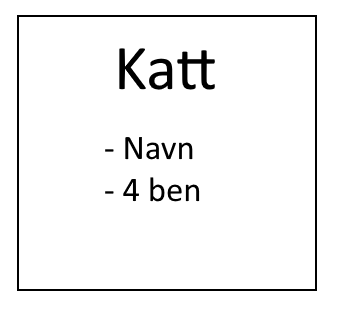
\includegraphics[scale=0.5]{Figures/Klasser_katt.png}
    \caption{En visualisering av klassen $"$Katt$"$.}
    \label{fig:Katte_boks}
\end{figure}

Når vi lager et rammeverk for alle kattene kan vi populere verdenen vår med mange katteobjekter. Det vil si at i verdenen vår har vi mange forskjellige katte-objekter, men alle katte-objektene tilhører klassen $"$Katt$"$ og hvert katte-objekt vil ha et navn og fire bein. Ved bruk av python som programmeringspråk skriver vi klassen for katt.\\[0.5cm]
\textbf{Del 1 (Kode):}
\begin{lstlisting}[language=python]
class Katt: #Klassen katt
    #Medlemsvariabler
    antall_ben = 4 
    navn ="" #Default navn
    
    #Constructor
    def __init__(self, navn): #Lager Katte-objektet med spesifisert navn
        self.navn = navn #Endrer navnet til katten fra "" til det vi spesifiserte

\end{lstlisting}
\textbf{Del 2 (Konsoll):}
\begin{lstlisting}[language=python]
>>> katten_butte = Katt("Butte") #Lager et katteobjekt med variabelnavn "katten_butte"
>>> print(katten_butte.navn) 
Butte
>>> print(katten_butte.antall_ben) 
4
\end{lstlisting}

En liten forklaring på hva som skjer.

$"$\twound{init}\twound{\text{ }}(self,navn)$"$ er en konstruktør for et katte-objektet. init kommer fra det engelske ordet $"$initial$"$. Når vi skal lage et et katteobjekt må vi kalle på konstruktøren vår. Ved å kalle på kontruktøren lager python et tomt objekt og sender det til oss i form av $"$self$"$. Self er på mange måter $"$Seg selv$"$ så når vi bruker self snakker vi om det spesifikke katte-objektet. Konstruktøren tar også inn et navn som vi må spesifiserer. Vi kunne også ha programmert konstruktøren til å ta inn antall bein også, men siden en katt alltid har 4 bein så gir det ingen mening å la brukeres bestemme hvor mange bein et katte-objektet skal ha. På linje 1 i Del 2 lager vi et objekt som vi kaller $"$katten\_butten$"$ som vi spesifiserer skal ha navnet $"$Butte$"$. Navn og antall bein til katten er en instans av klassen vår. Det vil si $"$Egenskaper$"$ til katte-objektet. Her er det viktig å skille mellom variabelnavnet på objektet og instansen til objektet som er vi har valgt å kalle $"$Navn$"$.

Sjefen vår er ikke helt fornøyd med at spillverdenen bare består av katter, han ber oss om å legge til hunder i tillegg og disse hundene skal kunne bjeffe.

\begin{figure}[H]
    \centering
    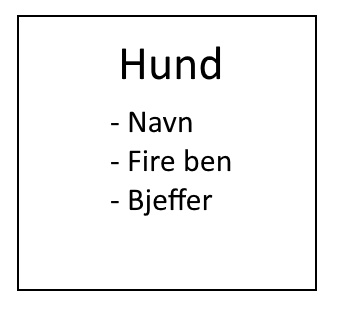
\includegraphics[scale=0.5]{Figures/Klasser_hund.png}
    \caption{En visualisering av klassen $"$Hund$"$.}
    \label{fig:klasse_hund}
\end{figure}

Hunden har mye av de samme instansene som en katt, men skal i tillegg ha en funksjonen å bjeffe. Dette gjør vi ved å lage det som kalles en medlemsfunksjon til klassen. En funksjon som bare klassen $"$Hund$"$ kan benytte seg av.\\[0.5cm]
\textbf{Del 1 (Kode):}
\begin{lstlisting}[language=python]
class Hund: #Klassen Hund
    #Medlemsvariabler
    antall_ben = 4 
    navn ="" #Default navn
    
    #Constructor
    def __init__(self, navn): #Lager hunde-objektet med spesifisert navn
        self.navn = navn #Endrer navnet til hunden fra "" til det vi spesifiserte
    #Medlemsfunksjon
    def bjeffe(self): 
        print("BARK BARK")
\end{lstlisting}
\textbf{Del 2 (Konsoll):}
\begin{lstlisting}[language=python]
>>> Hunden_tara = Hund("Tara") #Lager et Hundeobjekt med variabelnavn "Hunden_tara"
>>> print(Hunden_tara.navn) 
Tara
>>> Hunden_tara.bjeffe() #Kaller bjeffefunksjonen
BARK BARK
\end{lstlisting}

Nå har vi en klasse for Hund og for Katt som alle objekter i spillverdenen vår må følge. En klasse er et strengt rammeverket i form at et objekt kan ikke gjøre annet enn det klassen tillater. Det vil si at hvis vi prøver å skrive katten\_butte.bjeffe() så får vi feilmelding siden klassen Katt, som katten\_butte er et objekt av, ikke har en funksjon som heter bjeffe(). 


\subsection{Superklasser, subklasser og arv}
I mange tilfeller vil man ha klasser som har de samme medlemsvariablene og sammen medlemsfunksjonene. Istedet for å definere de samme funksjonene til hver klasse er det smartere å la en klasse arve medlemsfunksjoner og medlemsvariabler fra det vi kaller en superklasse. 

\subsubsection{Eksempel: Mange forskjellige dyr}
Sjefen vår kommer inn og sier at vi også skal ha kuer, griser, hester og mange andre forskjellige dyr i spillverdenen vår. Vi oppdager at dette blir mye repetisjon av kode som vi må spesifisere for hver klasse. Hund og katt hadde begge 4 ben og et navn. Her kan vi koble disse to klasse til en superklasse som vi kaller Dyr. Hund og Katt blir da subklasser av superklassen Dyr.

\begin{figure}[H]
    \centering
    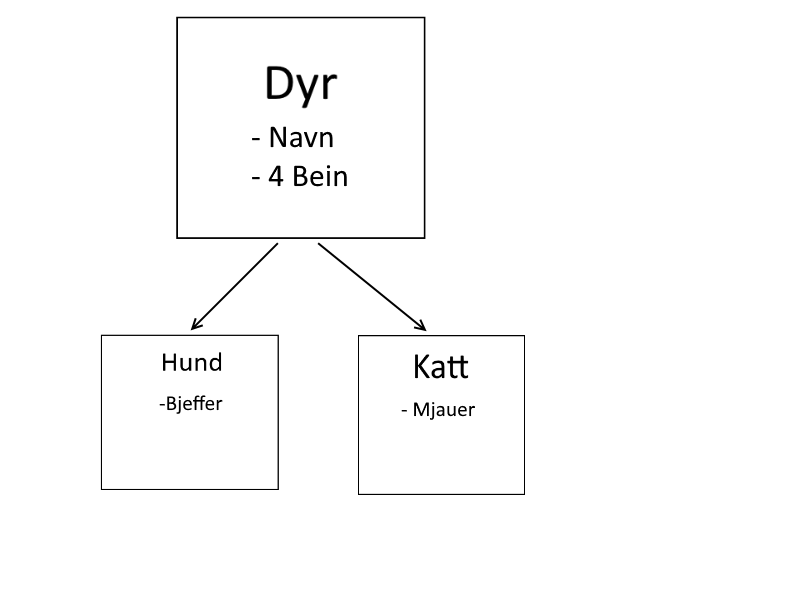
\includegraphics[scale=0.5]{Figures/Klasser_Dyr.png}
    \caption{En visualisering av superklassen Dyr med Katt og Hund som subklasser.}
    \label{fig:uperklasse}
\end{figure}
\begin{lstlisting}[language=python]
class Dyr(): # Klassen Dyr
    #Medlemsvariabler for alle dyre-objekter
    antall_ben = 4
    navn = ""
    #Contructor for dyre-objekter
    def __init__(self, navn):
        self.navn = navn

class Katt(Dyr): # Klassen Katt, arver fra klassen Dyr
    #Medlemsfunksjoner
    def mjaue(self):
        print("MJUAAAA")
        
    def __init__(self,navn): #Spesifiserer construktor for Katte-klassen
        super().__init__(self,navn) #Kaller superklassen sin constructor


class Hund(Dyr):  # Klassen Hund, arver fra klssen Dyr
    #Medlemsfunksjon
    def bjeffe(self):
        print("BARK BARK")
\end{lstlisting}

Som du ser i koden over så har klassen Katt en spesifisert konstruktør hvor av Hund har ingen. I realiteten er det ingen forskjell siden linje 15 kaller på konstruktøren til Dyr hvor av Katt vil automatisk kalle på den siden den arver konstroktøren til dyre-klassen. Linje 14 og 15 er med for å vise at man kan definere egne konstruktører for subklasser.

\textbf{Ekstra}: \\
Under er koden for filen $"$Min\_python\_fil.py$"$
\begin{lstlisting}[language=python]
if __name__ == "__main__":
    print("Dette er hovedskriptet")
\end{lstlisting}

Linje 1 i koden over er litt merkelig å forstå seg på, men tanken er at hvis du kaller på den spesifikke filen  $"$Min\_python\_fil.py$"$ så vil betingelsen til if-setningen gi ut True som gjør at linje 2 vil kjøre.

\begin{lstlisting}
>>> python Min_python_fil.py
Dette er hovedskriptet
\end{lstlisting}
 Vi ønsker å gjøre dette er fordi filen kan importeres fra andre filer. Hvis vi kjører en annen fil som importerer  $"$Min\_python\_fil.py$"$, så vil ikke if-betingelsen godkjennes.  

